\documentclass{beamer}

\input{../Haust2015glærur}

\title{Tölvunarfræði 1a}
\subtitle{Vika 11, fyrri fyrirlestur}

\begin{document}

\begin{frame}
\titlepage
\end{frame}

\section{Inngangur}

\begin{frame}{Í síðasta þætti\ldots}
\begin{itemize}
 \item Hreiðruð föll
 \item Endurkvæmni
\end{itemize}
Kaflar: 10.4 - 10.5
\end{frame}

\begin{frame}{Næstu skilaverkefni}
\begin{itemize}
 \item Útlit er fyrir að við náum 12 skilaverkefnum
 \begin{itemize}
  \item Skilaverkefni 9: Skil 3. nóvember
  \item Skilaverkefni 10: Skil 10. nóvember 
  \item Skilaverkefni 11: Skil 17. nóvember
  \item Skilaverkefni 12: Skil 24. nóvember - spes skil
 \end{itemize}
 \item Af þessum 12 verkefnum mun einkunn 10 bestu skilaverkefna gilda 20\% til lokaeinkunnar
\end{itemize}
\end{frame}

\section{Hlutbundin forritun}

\begin{frame}{Hlutbundin forritun}
\begin{itemize}
 \item Hingað til höfum við verið að raða gögnunum okkar niður í vigra, hólfafylki, færslur\ldots
 \begin{itemize}
  \item Föll taka gögnin síðan inn, vinna með þau og skila öðrum gögnum
  \item Þessi forritunaraðferð er oftast kölluð ``procedural programming''
 \end{itemize}
 \item Hægt er að nálgast forritun á annan hátt - hlutbundinn (e. \emph{object oriented})
 \begin{itemize}
  \item Hvaða fyrirbrigði/hlutir koma við sögu í vandamálinu?
  \item Hvernig hegða þessir hlutir sér?
 \end{itemize}
\end{itemize}
\end{frame}

\begin{frame}{Hvað er hlutur?}
\pause
\begin{itemize}
 \item Hvaða fyrirbrigði sem skilgreinast af gögnum og aðgerðum á þau geta verið hlutir
 \begin{itemize}
  \item Mjög opið hugtak! \pause
 \end{itemize}
 \item Dæmi um fyrirbrigði sem gætu verið hlutir í forriti \pause
 \begin{itemize}
  \item Allt sem sést í tölvuleikjum
  \item Hringur
  \begin{itemize}
   \item Gögn/eiginleikar: Staðsetning miðpunkts, radíus
   \item Aðgerðir: Teikna, reikna flatarmál
  \end{itemize} 
  \item Almennt brot
  \begin{itemize}
   \item Gögn/eiginleikar: Nefnari, teljari
   \item Aðgerðir: Leggja saman, stytta
  \end{itemize}
 \end{itemize}
\end{itemize}
\end{frame}

\section{Teiknihlutir}

\begin{frame}[fragile]{Teiknihlutir}
\begin{itemize}
 \item Fyrstu hlutirnir sem við sjáum í Matlab eru venjulega teiknihlutir
 \item Við getum skoðað teiknihlut með því að búa einn slíkan til
\begin{minted}{matlab}
>> f = figure
\end{minted}
 \item Getum fengið alla eiginleika hans með \texttt{get} fallinu
\begin{minted}{matlab}
>> get(f)
\end{minted}
\end{itemize}

\end{frame}


\section{Okkar eigin hlutir}

\begin{frame}[fragile]{Hvernig búum við til hluti í Matlab?}
\begin{columns}
\column{0.5\textwidth}
\begin{itemize}
 \item Til að búa til hluti í Matlab notum við svokallaða klasa (e. \emph{classes})
 \item Matlab-klasi á heima í sér \texttt{.m} skrá. Hann inniheldur
 \begin{itemize}
  \item Eiginleika (e. \emph{properties}) sem lýsa gögnum klasans
  \begin{itemize}
   \item Þetta eru breytur
  \end{itemize}
  \item Aðferðir (e. \emph{methods}) sem lýsa því hvernig gögnin hegða sér
  \begin{itemize}
   \item Þetta eru föll
  \end{itemize}
 \end{itemize}
\end{itemize}
\column{0.5\textwidth}
\begin{minted}[frame=lines]{matlab}
classdef ClassName % Nafn

    properties
        % Eiginleikar hingað
    end
    
    methods
        % Aðferðir hingað
    end
    
end
\end{minted}

\end{columns}
\end{frame}

\begin{frame}[fragile]{Dæmi: Almennt brot}
\begin{minted}[frame=lines, fontsize=\small]{matlab}
classdef Fraction

    properties
        n % Teljari / numerator
        d % Nefnari / denomenator
    end
    
    methods
        function frac = Fraction(numerator, denomenator)
            frac.n = numerator;
            frac.d = denomenator;
        end
    end
    
end
\end{minted}

\end{frame}

\begin{frame}{Í Matlab}
\begin{center}
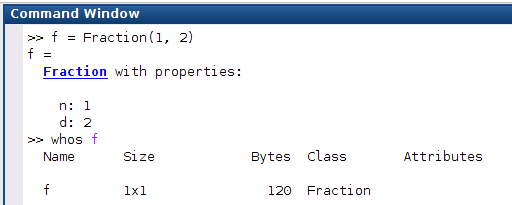
\includegraphics[width=\textheight]{Pics/fraction-workspace}
\end{center}
\end{frame}


\begin{frame}{Hvað vorum við að horfa á?}
\begin{itemize}
 \item Við vorum að skoða klasa með\ldots
 \item Tveimur eiginleikum
 \begin{itemize}
  \item \texttt{n} og \texttt{d}, sem tákna teljara og nefnara
  \item Einni aðferð, sem ``smíðar'' nýja hluti
  \begin{itemize}
   \item Slík aðferð er kölluð smiður (e. \emph{constructor})
   \item Notuð til að upphafsstilla gildi, athuga hvort að breyturnar séu af leyfilegum gerðum o.fl.
   \item Flestir klasar hafa smið
  \end{itemize}
 \end{itemize}
\end{itemize}
\end{frame}

\begin{frame}[fragile]{Fleiri aðferðir}
\begin{columns}
\column{0.45\textwidth}
\begin{itemize}
 \item Til að klasinn okkar virki vel þarf hann fleiri aðferðir
 \item Oftast viljum við að klasinn okkar prentist á skynsamlegan hátt út þegar við köllum á \texttt{disp} eða þegar við gefum breytum gildi af hans tagi
 \item Hvernig gerum við það?
 \begin{itemize}
  \item Bætum við \texttt{disp} aðferð á klasann!
 \end{itemize}
\end{itemize}
\column{0.55\textwidth}

\begin{minted}[frame=lines, fontsize=\small]{matlab}
function disp(fr)
    fprintf('%d/%d\n', fr.n, fr.d)
end
\end{minted}

Þetta fer inn í ``\texttt{methods}'' blokk klasans
\end{columns}
\end{frame}

\begin{frame}[fragile]{Látum klasann vinna vinnu}
\vspace{\baselineskip}
Við kunnum að leggja saman brot:
\[
\frac{c}{d} + \frac{a}{b} = \frac{cb+ad}{db} 
\]
Þetta má gera í klasanum okkar með því að bæta við aðferðinni
\begin{minted}[frame=lines]{matlab}
function newFrac = add(frac1, frac2)
    newN = frac1.n * frac2.d + frac2.n * frac1.d;
    newD = frac1.d * frac2.d;
    newFrac = Fraction(newN, newD);
end
\end{minted}
\end{frame}

\begin{frame}[fragile]{Af hverju hlutbundin forritun?}
\begin{itemize}
 \item Mörgum ``kerfum'' er auðvelt að lýsa með hlutbundnum aðferðum
 \begin{itemize}
  \item Sérstaklega kerfum sem eiga að herma eftir bókstaflegum hlutum
 \end{itemize}
 \item Ýmis atriði í hlutbundinni forritun hjálpa til við að gera kóða endurnýtanlegan og skilanlegri
 \begin{itemize}
  \item Erfðir, hjúpun, \ldots
 \end{itemize}
\end{itemize}
\end{frame}

\begin{frame}{Fyrirlestraræfing}
\begin{enumerate}
 \setcounter{enumi}{3}
 \item Breytið \texttt{disp} aðferðinni í \texttt{Fraction} klasanum okkar svo að tölur með 1 í nefnara séu sýndar án nefnara (t.d. sýna töluna \texttt{3} en ekki \texttt{3/1})
 \item Bætið margföldunaraðferð við \texttt{Fraction} klasann
\end{enumerate}

\end{frame}


\end{document}
